\documentclass{article}
\usepackage{amsmath}
\usepackage{amssymb}
\usepackage{algorithm}
\usepackage{float}
\usepackage{color}
\usepackage{multicol}
\usepackage{forloop}
\usepackage{graphicx}
\usepackage[margin=0.8in]{geometry}
\usepackage{caption}
\usepackage{enumerate}
\graphicspath{ {.} }
\title{STAT 2509B4 \\
	\large{Assignment 2}}
\author{Krystian Wojcicki, 101001444}
\date{Winter 2020}

\begin{document}
\maketitle


Indicate whether or not each of the following models can be treated as an multiple linear
regression (MLR) model:
\begin{enumerate}[(i)]

\item  $y = \beta_0 + \beta_1x_1 + \beta_2x_2 + \beta_3x_1x_2 + \epsilon $, can be treated as MLR
\item  $y = (e^{\beta_0 + \beta_1x_1 + \beta_2x_2^2})\epsilon$, cannot be treated as MLR
\item  $y = \beta_0 + \beta_1x_1 + \beta_2e^{x_1} + \epsilon$, can be treated as MLR
\item  $y = \beta_0 + \beta_1x_1 + \beta_2x_1^2 + \beta_3x_1^3 + \beta_4x_2 + \epsilon$, can be treated as MLR
\item $y = \beta_0e^{\beta_1x_1 + \beta_2x_2} + \epsilon$, cannot be treated as MLR

\end{enumerate}

\begin{enumerate}[(a)]
\item \textbf{State all the assumptions that are necessary for the statistical inference under the MLR model.: } \\
Model $y = \beta_0 + \beta_1x_1 + \beta_2x_2 + \epsilon, n = $ TODO \\
Assumptions
  \begin{enumerate}[(1)]
   \item $X_1, X_2$ are observed without error
   \item $\epsilon$'s are independently distributed
   \item $\epsilon$'s have common mean 0 in other words $E(\epsilon) = 0$ for all $X_1,X_2$.
   \item $\epsilon$'s have common/constant variance $\sigma^2$ meaning $Var(\epsilon) = \sigma^2$ for all $X_1,X_2$
  \item $\epsilon \sim N(0, \sigma^2)$ for any value of $X_1, X_2$
\end{enumerate}

\item \textbf{Use matrices to compute the least-squares estimates of the population parameters $\beta_0$, $\beta_1$ and $\beta_2$, and obtain the fitted least-squares regression line:  \\
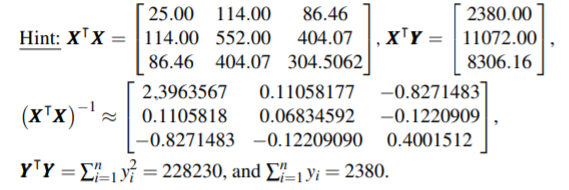
\includegraphics{a3_hint}} \\

$(X^TX)^{-1} X^TY = \begin{bmatrix}
2.3963567 & 0.11058177 & -0.8271483 \\
0.1105818 & 0.06834592 & -0.1220909 \\
-0.8271483 & -0.12209090 & 0.400151 \\
\end{bmatrix} * 
\begin{bmatrix}
2380.00 \\
11072.00 \\
8306.16 \\
\end{bmatrix}= 
\begin{bmatrix}
57.2642 \\
5.80416 \\
3.31483 \\
\end{bmatrix} = 
\begin{bmatrix}
    \hat{\beta_0} \\
    \hat{\beta_1} \\
    \hat{\beta_2}
\end{bmatrix} = \hat{\beta}$


\item \textbf{ Set up the ANOVA table and test for significance of the model at the significance level of $\alpha$ = 0.05 } \\
$TSS = Y^TY - \frac{(\sum_{i=1}^{n}{y_i})^2}{n} = \sum_{i=1}^{n}{y_i^2} - \frac{(\sum_{i=1}^{n}{y_i})^2}{n}  = 228230 - \frac{2380^2}{25} = 1654$

$SSR = \hat{\beta^T}(X^TY)  - \frac{(\sum_{i=1}^{n}{y_i})^2}{n}  = \begin{bmatrix}
57.2642 & 5.80416 & 3.31483
\end{bmatrix} * \begin{bmatrix}
2380.00 \\
11072.00 \\
8306.16 \\
\end{bmatrix} - \frac{2380^2}{25} = 1509.9638728$

$SSE = TSS - SSR = 1654 - 1509.9638727 = 144.0361272$
$MSR = \frac{SSR}{k} = \frac{1509.9638728}{2} = 754.9819364$
$MSE = \frac{SSE}{n-(k+1)} = \frac{144.0361272}{22} = 6.547$
$F = \frac{MSR}{MSE} = \frac{754.9819364}{6.547} = 115.317$

\begin{center}
 \begin{tabular}{||c c c c c||} 
 \hline
Source & d.f & SS & MS & F \\ [0.5ex] 
 \hline\hline
Regression & 2 & 1509.9638728 & 754.9819364 & 115.317 \\
 \hline
Error & 22 & 144.0361272 &  6.547 &  \\
 \hline
Total & 24  & 1654 & & \\ [1ex]
 \hline
\end{tabular}
\end{center}

$H_0: \beta_1 = \beta_2 = 0$ \\
$H_a: \text{at least one of the } \beta's \neq 0$ \\
$\alpha = 0.05$

test-statistics: $F = \frac{MSR}{MSE} = 115.317$

Rejection region, we rejected $H_0$ if $F > F_{(k, n-(k+1)), \alpha} = F_{2, 22; 0.05} = 3.4434$

Since $F = 115.317 > 3.4434$, we reject $H_0$ and conclude that at a 5\% level of significance there is evidence to say there is a linear relationship between age, weight and the systolic BP.

\item \textbf{ Test whether age (x1) contributes to explaining (or predicting) the systolic blood pressure (y) under the MLR model. Use t-test with $\alpha = 0.05$. } \\

$H_0: \beta_1 = 0$
$H_a: \beta_1 \neq 0$
$\alpha = \to \alpha/2 =  $

test statistics: $t = \frac{\hat{\beta_1}}{\sqrt{v_{11}MSE}} = \frac{5.80416}{\sqrt{0.0683459 * 6.547}} = 8.677$

Rejection region, we reject $H_0$ if $|t| > t_{n-(k+1), \alpha/2} = 2.07383$.

Since $t = 8.677 > 2.07$, we reject $H_0$ and conclud that at a 5\% level of significance there is evidence to say that the $x_1$ term contributes to the model.

\item \textbf{ Find the values of the coefficient of determination, $r^2$, and the adjusted $r^2$. Interpret their meanings in this problem} \\

$r^2 = \frac{SSR}{TSS} = \frac{1509.9638727}{1654} = 0.9129 = 91.29\%$

In other words approximately 91.29\% of the total variation in the data is explined by the regression line. The rest is due to error.

$r_{adj}^2 = 1 - \frac{SSE/n-(k+1)}{TSS/n-1} = 1 - \frac{MSE}{TSS/n-1} = 1 - \frac{6.547}{1654/24} = 0.9050 = 90.50\%$

Since both $r^2$ and $r_{adj}^2$ are quite high, around 90\%, and since the $x_1$ term does contribute to the model, we can conclude that the model is good.

\item \textbf{ Run SAS to verify your answers to the above questions. In addition, use the SAS output to answer subquestion (d) using the partial F-test with $\alpha$ = 0.05.} See attatched SAS output

$H_0: \beta_1 = 0$
$H_a: \beta_1 \neq 0$
$\alpha = 0.05$

full model: $y = \beta_0 + \beta_1x_1 + \beta_2x_2 + \epsilon$
reduced model: $y = \beta_0 + \beta_2x_2 + \epsilon$

test statistics:
$F_{part} = \frac{ [SSR_f - SSR_r] / [df_{SSR_f} - df_{SSR_r} ] }{ SSE_f / df_{SEE_f} } = $

Rejection Region, we reject $H_0$ if $F_{part} > F_{(1, 22); 0.05 = TODO$

\end{enumerate}


$y = \beta_0 + \beta_1x_1 + \beta_2x_2 + \beta_3x_3 + \beta_4x_1x_2 + \beta_5x_1x_3 + \epsilon$

Full mode: $y = \beta_0 + \beta_1x_1 + \beta_2x_2 + \beta_3x_3 + \beta_4x_1x_2 + \beta_5x_1x_3 + \epsilon$

If drug A: $y = \beta_0 + \beta_1x_1 + \epsilon$

If drug B: $y = \beta_0 + \beta_1x_1 + \beta_2 + \beta_4x_1 \epsilon$

If drug C: $y = \beta_0 + \beta_1x_1 + \beta_3 + \beta_5x_1 + \epsilon$

Test if any of the 3 drug lines are parallel or have the same slope
$H_0: \beta_4 = \beta_5 = 0$
$H_a:$ at least one of the $\beta$'s $neq 0$.
$\alpha = 0.05$

Reduce model

\begin{enumerate}[1.]
\item

\textbf{ A medical study was conducted to study the relationship between infants’ systolic blood
pressure and two explanatory variables, age (days) and weight (kg). The data for 25 infants
are given below..:\\
\begin{center}
 \begin{tabular}{||c c c||} 
 \hline
Age ($x_1)$ & Treadmill time in minutes ($x_2$) & Systoli BP (y) \\ [0.5ex] 
 \hline\hline
3 & 2.61 & 80 \\
\hline
4 & 2.67 & 90 \\
\hline
5 & 2.98 & 96\\
\hline
6 & 3.98 & 102\\
\hline
3 & 2.87 & 81\\
\hline
4 & 3.41 & 96\\
\hline
5 & 3.49 & 99\\
\hline
6 & 4.03 & 110\\
\hline
3 & 3.41 & 88\\
\hline
4 & 2.81 & 90\\
\hline
5 & 3.24 & 100\\
\hline
6 & 3.75 & 102\\
\hline
3 & 3.18 & 86\\
\hline
4 & 3.13 & 93\\
\hline
5 & 3.98 & 101\\
\hline
6 & 4.55 & 103\\
\hline
3 & 3.41 & 86\\
\hline
4 & 3.35 & 91\\
\hline
5 & 3.75 & 100\\
\hline
6 & 3.83 & 105\\
\hline
3 & 3.18 & 84\\
\hline
4 & 3.52 & 91\\
\hline
5 & 3.49 & 95\\
\hline
6 & 3.81 & 104\\
\hline
6 & 4.03 & 107  \\ [1ex]
 \hline
\end{tabular}
\end{center}
}
\begin{enumerate}[(a)]
  \item \textbf{Draw a scatter plot (using SAS, see part (i)) to get an idea of the form of the relationship
between the treadmill time (x) and 10-km running time (y). Does the scatter plot suggest
an approximate linear relationship between the two variables?: }
See SAS output attatched \\
  \item \textbf{State a simple linear regression (SLR) model for two variables and describe all assumptions that are necessary for statistical inference.
: } \\
Model $y = \beta_0 + \beta_1 * x+ \epsilon, n = 20$.
Assumptions
  \begin{enumerate}[(1)]
   \item The random errors $\epsilon_i$'s are mutually independent.
   \item $\epsilon_i$'s are normally distributed
   \item $\epsilon_i$'s have common mean 0 in other words $E(\epsilon_i) = 0$ for all $i$.
   \item $\epsilon_i$'s have common variance $\sigma^2$ meaning $Var(\epsilon_i) = \sigma^2$ for all $i$
  \item $x$'s are observed without error.
\end{enumerate}
  \item \textbf{Find the least squares estimates of $\beta_0$ and $\beta_1$ in the SLR model. Find the least square
fitted regression line.: } \\
\begingroup
\Large
\begin{equation}
\hat{\beta_1} = \frac{S_{xy}}{S_{xx}} = \frac{  \sum_{i=1}^{n}{x_iy_i }  - \frac{  \sum_{i=1}^{n}{x_i}  \sum_{i=1}^{n}{y_i}  }{n} }
{  \sum_{i=1}^{n}{x_{i}^2} - \frac{    (\sum_{i=1}^{n}{x_i})^2    }{ n }}   = \frac{ 7852.25 - \frac{195.1 * 812}{20}  }{ 1940.05 - \frac{(195.1)^2 }{20} }  = -1.8673252 \simeq -1.87  \nonumber
\end{equation}
$\hat{\beta_0} = \bar{y} - \hat{\beta_1}\bar{x} = \frac{ \sum_{i=1}^{n}{y_i} }{n} - \hat{\beta_1}\frac{\sum_{i=1}^{n}{x_i} }{n} = \frac{812}{20} + 1.87 * \frac{195.1}{20} = 58.815757 \simeq 58.82 $
\endgroup
Therefore the least square fitted regression is given by $\hat{y} = 58.82 - 1.87x$ 

\item \textbf{Find $s^2$, an estimate of $\sigma^2$: } \\

\begingroup
\Large
$s^2 = \frac{SSE}{n-2} = \frac{S_{yy} - \frac{S_{xy}^2}{S_{xx}}}{n-2} = \frac{            (\sum_{i=1}^{n}{y_i^2} - \frac{ (\sum_{i=1}^{n}{y_i})^2}{n} )  - 
\frac{   ( \sum_{i=1}^{n}{x_iy_i }  - \frac{  \sum_{i=1}^{n}{x_i}  \sum_{i=1}^{n}{y_i}  }{n})^2     }
{    (\sum_{i=1}^{n}{x_i^2} - \frac{ (\sum_{i=1}^{n}{x_i})^2}{n} )     }}
{n - 2}$ \\
$ = \frac{ (33175.2 - \frac{812^2}{20}) - \frac{ (7852.25 - \frac{195.1 * 812}{20})^2}{1940.05-\frac{195.1^2}{20}}  }{18} = \frac{208 - 128.49}{18} = 4.41718627269 \simeq 4.42 $
\endgroup

Therefore $s = \sqrt{s^2} = \sqrt{4.42} = 2.10171032083 \simeq 2.10$

  \item \textbf{Use the t-test to test whether there is a significant linear relationship between 10-km
running time and the treadmill time. Use $\alpha$ = 0.05.: }

$H_0: \beta_1 = 0, H_a: B_1 \neq 0$ \\
$\alpha = 0.05 \to \alpha/2 = 0.025$

Since we are using a t-test, our test statistic is t and $t= \frac{\hat{\beta_1} - 0}{s/\sqrt{S_{xx}}} = \frac{-1.87}{2.10/\sqrt{36.8495}} = -5.3934 \simeq -5.39$

Rejection region, we reject $H_0$ if $|t| > t_{n-2;\alpha/2} = t_{18;0.025} = 2.101$

Since $|t| = |-5.39| = 5.39 > 2.101$, we reject $H_0$ and we can conclude that at $\alpha = 0.05$ or 5\% level of significance there is evidence that there is a linear relationship between 10-km running time and the treadmill time.

  \item \textbf{ Find a 95\% confidence interval for $\beta_1$.: }

$1 - \alpha = 0.95 \to \alpha = 0.05 \to \alpha/2 = 0.025$

Therefore $\beta_1$'s 95\% confidence interval is \\ 
$(\hat{\beta_1} \pm t_{n-2;\alpha/2}\frac{s}{\sqrt{S_{xx}}}) = (-1.87 \pm 2.101 * \frac{2.10}{\sqrt{36.85}}) = (-2.59474163696, -1.13990876535) \simeq (-2.60, -1.14) $. And we can be 95\% confident that in repeated sampling the true value of $\beta_1$ would lie in the interval $(-2.60, -1.14)$.

  \item \textbf{ Set up the ANOVA table and use it to test whether there is a significant linear relationship between 10-km running time and the treadmill time. Use $\alpha$ = 0.05.: }

$TSS = S_{yy} = \sum_{i=1}^{n}{y_i^2} - \frac{ (\sum_{i=1}^{n}{y_i})^2 }{n} = 33175.2 - \frac{812^2}{20} = 208 $ \\
$SSR = \frac{S_{xy}^2}{S_{xx}} = \frac{ (7852.25 - \frac{195.1 * 812}{20})^2}{ 1940.05 - \frac{195.1^2}{20}} = 128.49 $ \\
$SSE = TSS - SSR = 208 - 128.49 = 79.51 $ \\ 
$MSR = SSR/1 = 128.49 $ \\ 
$MSE = \frac{SSE}{n-2} = \frac{79.51}{18} = 4.42$ \\
$F = \frac{MSR}{MSE} = \frac{128.49}{4.42} =  29.09 $ \\

\begin{center}
 \begin{tabular}{||c c c c c||} 
 \hline
Source & d.f & SS & MS & F \\ [0.5ex] 
 \hline\hline
Regression & 1 & 128.49 & 128.49 & 29.09 \\
 \hline
Error & 18 & 79.51 & 4.42 &  \\
 \hline
Total & 19  & 208 & & \\ [1ex]
 \hline
\end{tabular}
\end{center}

$H_0: \beta_1 = 0, H_a: \beta_1 \neq 0$
With $\alpha = 0.05$.

Using F-test so statistic is $F = \frac{MSR}{MSE} = 29.09$

Rejection region, we reject $H_0$ if $F > F_{1,n-2;\alpha} = F_{1,18;0.05} = 4.41$.

Since $F = 29.09 > 4.41$ we can reject $H_0$ and conclude that at a 5\% level of significance there is evidence of a linear relationship between the 10-km running time and the treadmill time. 

  \item \textbf{ Find the values of the coefficient of correlation, r, and the coefficient of determination,$r^2$, and interpret their meaning in this problem.: }

$r = \frac{S_{xy}}{\sqrt{S_{xx}S_{yy}}} = \frac{7852.25-\frac{195.1*812}{20}}{\sqrt{ (1940.05 - \frac{195.1^2}{20}) * (33175.2-\frac{812^2}{20})}} = -0.785966599565 \simeq -0.79$ \\

Therefore the 10-km running time and the treadmill time are quite strongly negatively correlated with the strength of their relationship close to 78.60\%.

$r^2 = \frac{SSR}{TSS} = \frac{128.49}{208} = 0.617740384615 \simeq 0.62$ \\

Therefore approximately 61.77\% of the total variation in the data can be explainded by the regression line and the remaining \% is due to error. And conclusion that the model is a good fit to the data as $r^2 > 50\%$

  \item \textbf{Verify your results for (b) to (h) using SAS.}
See SAS output attatched


\end{enumerate}

\item \textbf{Refer to Question 1.}
\begin{enumerate}[(a)]
\item \textbf{Find a 95\% confidence interval for the mean
value of the response variable (i.e. the 10-km running time) and a 95\% prediction
interval for an individual value of the response variable when the treadmill time is 9.5
minutes. What can you say about the widths of these two intervals.:}


95\% confidence interval for $E(y)$ when $x_p =9.5$. 

$\hat{y} = 58.82 - 1.87(9.5) = 41.055$ and since $1 - \alpha \to 0.95 \to \alpha = 0.05 \to \alpha/2 = 0.025$

Therefore $E(9.5)$ falls into the interval \\
$(\hat{y} \pm t_{n-2;\alpha/2} * s * \sqrt{ \frac{1}{n} + \frac{(x_p - \bar{x})^2}{S_{xx}}}) = (41.06 \pm 2.101 * 2.10 * \sqrt{\frac{1}{20} + \frac{(41.06 - 9.755)^2}{ 1940.05 - \frac{195.1^2}{20}} }) = (39.9953486251, 42.0646513749) \simeq (40.00, 42.07)$. So we are 95\% confident that after repeating sampling the mean value of the 10-km running time when the treadmill time is 9.5 minutes would fall in the interval $(40.00, 42.07)$. \\

95\% prediction interval for $y$ when $x_p = 9.5$

Therefore $y$ falls into the interval \\
$(\hat{y} \pm t_{n-2;\alpha/2} * s * \sqrt{ 1+ \frac{1}{n} + \frac{(x_p - \bar{x})^2}{S_{xx}}}) = (41.06 \pm 2.101 * 2.10 * \sqrt{1 + \frac{1}{20} + \frac{(41.06 - 9.755)^2}{ 1940.05 - \frac{195.1^2}{20}} }) = \\
(36.4714602301, 45.5885397699) \simeq (36.47, 45.59)$. So we are 95\% confident that after repeating sampling the vaue of the 10-km running time when the treadmill time is 9.5 minutes would fall in the interval $(36.47, 45.59)$. \\

The P.I is wider than the C.I. this is expected as the variability in the error for predicting a single value is greater than the variability of error for the estimation of the mean or average value of y.

\item \textbf{Use SAS to answer subquestion 2(a) and compare your SAS results to your handcalculated results. (See Part (c) of the SAS example.)}

See SAS output attatched.

\end{enumerate}

\item \textbf{Perform a residual analysis to check the SLR model assumptions using SAS (see Part (b) of
the SAS example). What can you conclude?}

\end{enumerate}

\begin{center}
	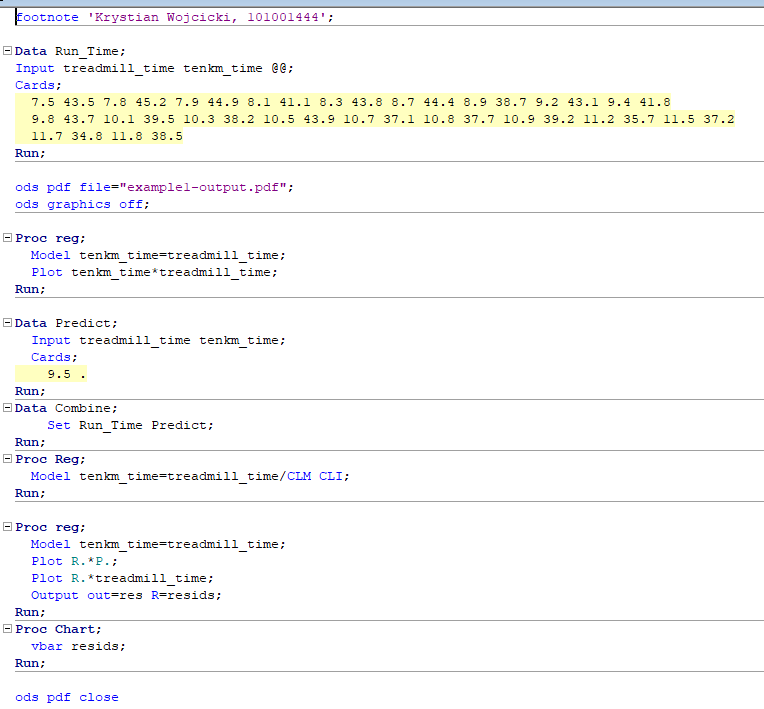
\includegraphics{a2_sascode}
\end{center}

\end{document}